\documentclass[a4paper,11pt,twoside,openright,english]{article}
\usepackage{babel,epsfig,amssymb,amsmath,amsthm,wasysym,pifont,latexsym,rotating,setspace}
\usepackage{graphicx}
\usepackage[utf8]{inputenc}
\usepackage{listings}
\usepackage{float}
\usepackage{multirow,bigdelim}
\usepackage{color}
\usepackage{longtable}
\usepackage{hyperref}
\usepackage{tikz}
\usetikzlibrary{shapes.geometric,arrows.meta,positioning,fit,backgrounds}
\definecolor{dkgreen}{rgb}{0,0.6,0}
\definecolor{gray}{rgb}{0.5,0.5,0.5}
\definecolor{mauve}{rgb}{0.58,0,0.82}
\pagestyle{plain}
\topmargin -0.5cm
\oddsidemargin 0cm
\evensidemargin 0cm
\textwidth 16cm
\textheight 24cm

\lstset{frame=tb,
  language=bash,
  aboveskip=3mm,
  belowskip=3mm,
  showstringspaces=false,
  columns=flexible,
  basicstyle={\small\ttfamily},
  numbers=none,
  numberstyle=\tiny\color{gray},
  commentstyle=\color{dkgreen},
  stringstyle=\color{mauve},
  breaklines=true,
  breakatwhitespace=true,
  tabsize=3
}

\newcommand{\specialcell}[2][c]{%
  \begin{tabular}[#1]{@{}c@{}}#2\end{tabular}}

\tikzset{
  startstop/.style={rectangle, rounded corners, minimum height=0.9cm, minimum width=3.2cm,
    text width=3.0cm, align=center, draw=black, fill=orange!25, font=\small},
  process/.style={rectangle, minimum height=0.9cm, minimum width=4.2cm,
    text width=4.0cm, align=center, draw=black, fill=blue!12, font=\small},
  mesonh/.style={rectangle, minimum height=0.9cm, minimum width=4.2cm,
    text width=4.0cm, align=center, draw=black, fill=gray!18, font=\small},
  decision/.style={diamond, aspect=2.2, minimum height=0.9cm, minimum width=3.6cm,
    text width=2.3cm, align=center, draw=black, fill=yellow!25, font=\scriptsize, inner sep=1pt},
  wkarrow/.style={-{Latex[length=2mm]}, thick},
  wknote/.style={rectangle, minimum height=0.7cm, text width=3.6cm, align=center,
    draw=black, dashed, fill=green!8, font=\scriptsize}
}

\begin{document}

\begin{center}
  \begin{LARGE}
    \textbf{FAST AUTOMATION MODULE}\\
    \textbf{MANUAL}\\
  \end{LARGE}
  \vspace{1cm}
  \begin{footnotesize}
    \textbf{Generic single-configuration edition}\\
    \textbf{\today}\\
  \end{footnotesize}
  \vspace{1cm}
\end{center}

\tableofcontents
\newpage

\section{INTRODUCTION}

This manual describes the \textbf{automation module} of \textbf{FAST} (Forecast Automation System for
Telescopes), the component that runs a single, once-per-night Meso-NH / Astro-Meso-NH atmospheric and
optical-turbulence forecast for a ground-based telescope site. It automates the full chain: waiting for
and validating the initialization files, running the mesoscale simulation, post-processing the raw
model output into astroclimatic parameters, generating diagnostic plots, and delivering the results to
a remote server.

This document describes the automation \emph{generically}, i.e.\ independently of the specific
telescope, site or forecasting project it is deployed for. FAST has been deployed, in slightly
different configurations, for more than one ground-based observatory; this manual covers the common
core that any such deployment shares, not the site-specific choices (domain geometry, delivered file
formats, calibration constants) that a given installation layers on top of it via its own
\texttt{conf.d/*.var} files. Where a parameter table below shows a \texttt{[current: ...]} value, that
value is simply whatever this particular installation's configuration files currently contain, given as
a worked example -- not a universal default.

This document covers only the \emph{automation} part of FAST, i.e.\ the component that produces the
once-per-night Meso-NH forecast. A separate, complementary \emph{short-timescale} component (an
autoregressive or machine-learning correction of the forecast using real-time telemetry, updated every
few minutes) may run alongside it on some deployments; it is a distinct program with its own
configuration and is documented separately. Section~\ref{sec:usage} describes the point at which the
automation hands data off to it, where applicable.

The user of this manual is assumed to be familiar with the basic operation of Meso-NH, with the Linux
shell, and with basic bash scripting. A working installation of Meso-NH and of a local OpenMPI build is
assumed to already be in place; Section~\ref{sec:deps-install} lists the remaining dependencies and the
steps needed to install and configure the automation code on top of them.

\textbf{Scope of this revision.} This is a \emph{single-configuration} edition of the manual: it
documents one self-contained instance of the automation (one \texttt{bin/} tree, one set of
\texttt{conf.d/*.var} files, one nightly \texttt{run.sh}), started directly (by cron or manually) with
no external orchestration layer coordinating multiple instances or deciding which one's output to keep.
Deployments that do chain several configurations together (for example, running a second, different-
resolution configuration after the first, or driving several instances from a shared top-level script)
require that coordination layer to be documented separately, on top of this manual; nothing here
describes it.

\textbf{A note on scope.} This manual documents what the automation does and how it is configured; it
assumes solid Linux system administration and shell-scripting skills, and it is not a substitute for
them. In an operational deployment, reading the source code directly -- not just this manual -- is
eventually unavoidable: some situation not covered here will arise, and resolving it will require
understanding the scripts themselves. No manual can substitute for the operational experience needed to
run an unattended automated system in production; that experience is built on the job, by encountering
and working through real problems as they occur.

\section{SYSTEM ARCHITECTURE AND WORKFLOW}
\label{sec:usage}

\subsection{Overview}
This edition of the automation runs \textbf{one Meso-NH configuration, once per night}: a single set of
nested domains (\texttt{NESTING} in \texttt{globals.var}, currently 3 -- outer domain plus two nested
levels), driven by one self-contained \texttt{bin/} tree and one \texttt{bin/conf.d/*.var} configuration
(Section~\ref{sec:config}). There is no built-in mechanism in this codebase for running several
configurations in sequence or for having one run's output conditionally replace another's; if a
deployment needs that (e.g.\ a coarser and a finer-resolution configuration chained together), it has to
be implemented as an external wrapper around this code, and documented separately.

\subsection{Manual and scheduled operation}
The whole procedure is a single entry point, \texttt{bin/run.sh}, invoked with no arguments:
\begin{lstlisting}
cd bin
./run.sh
\end{lstlisting}
For nightly unattended operation this is normally launched from cron, e.g.:
\begin{lstlisting}
0 20 * * * /path/to/bin/run.sh > /path/to/sim.out 2>&1
\end{lstlisting}
\texttt{run.sh} locates its own configuration via \texttt{conf.d/globals.var} relative to its own path,
so it must be run from within \texttt{bin/} (or by an absolute path that still resolves correctly). The
date being processed is controlled by \texttt{YEAR}/\texttt{MONTH}/\texttt{DAY} in \texttt{times.var}
(Section~\ref{sec:config}): under normal operation these are meant to track ``today'' (they default to
the system date at the top of the file), but \textbf{a hand-set override further down the file
currently takes precedence} -- see the note in Section~\ref{sec:config} on \texttt{times.var}. To
process a specific night (whether for the scheduled run or for manual reprocessing of a past date), edit
that override directly. There is no external process that substitutes today's date into the
configuration automatically; whatever \texttt{times.var} contains at the time \texttt{run.sh} sources it
is what gets used.

\subsection{Workflow (\texttt{run.sh})}
\texttt{bin/run.sh} performs, in order:
\begin{enumerate}
  \item \textbf{Startup}: kills any leftover Meso-NH-related processes from a previous, possibly stuck
        run (\texttt{pkill} on the executable names from \texttt{globals.var}), rotates the log
        directory, and sources \texttt{times.var} then \texttt{run.var}.
  \item \textbf{Initialization file retrieval}: sources \texttt{filedef.var} directly -- \textbf{this is
        where the actual wait happens}, in \texttt{run.sh}'s own process. \texttt{filedef.var}'s logic
        waits for the raw initialization files for the requested forcing hours to appear in
        \texttt{INIRAWDIR}, retries downloading them from a configurable backup server over SSH if they
        are late or missing, verifies each file's MD5 checksum, and merges the orography information
        from the analysis file into each forecast file with \texttt{grib\_copy} -- aborting with an
        alert mail if the files still have not arrived after a configurable timeout (\texttt{TIMELIMIT}
        in \texttt{times.var}). \texttt{run.sh} then sources \texttt{backup.var}.
  \item \textbf{Reference script generation}: only once the previous step has confirmed the
        initialization files are present, and only if \texttt{TESTRUN=0} and \texttt{PREPLISTTRUE=1}
        (and \texttt{NOPREP=0}\slash\texttt{NORUN=0}), \texttt{run.sh} invokes \texttt{bin/prep\_list.sh} as
        a sub-process. As explained in full in Section~\ref{sec:executables},
        \texttt{prep\_list.sh}'s own purpose is to generate a pair of self-contained, legacy-style
        reference scripts, not to fetch files; it re-sources \texttt{filedef.var} itself (in its own,
        separate shell) purely to know which files to write into those scripts, and since they are
        already present by this point, this second sourcing does not itself wait on anything.
        \texttt{run.sh} then moves the two generated scripts into \texttt{LOGDIR}.
  \item \textbf{PREP\_REAL phase}: for every nested domain, runs Meso-NH's \texttt{PREP\_REAL\_CASE}
        (and \texttt{SPAWNING} for nested domains) to build the initial and boundary conditions.
  \item \textbf{EXE phase}: runs the \texttt{MESONH} executable under \texttt{mpirun}, producing the
        raw \texttt{.lfi} model output for the whole forecast segment.
  \item \textbf{POSTPROC phase} (\texttt{bin/postproc.sh}, sourced): runs the \texttt{DIAG} step and
        \texttt{conv2dia}\slash\texttt{diaprog} to derive the astroclimatic parameters (optical
        turbulence $C_N^2$ and integrated parameters, wind, temperature, relative humidity, PWV, etc.)
        and to extract them as ASCII (FICVAL vertical profiles/cuts and 2D ground maps) at the points,
        domains and heights configured in \texttt{run.var}.
  \item \textbf{PLOT phase} (\texttt{bin/plot\_python.sh}, sourced): runs the Python plotting suite
        under \texttt{bin/conf.d/utils/Plot\_python/} (one script per parameter/plot type) to turn the
        ASCII output into the delivered figures.
  \item \textbf{Compression}: optionally \texttt{bzip2}-compresses the raw PREP\_REAL, RUN and DIAG
        \texttt{.lfi} outputs in parallel (GNU \texttt{parallel}), controlled by
        \texttt{DOZIPREAL}\slash\texttt{DOZIPOUT}\slash\texttt{DOZIPDIAG} in \texttt{globals.var}.
  \item \textbf{Move to staging}: moves the outputs selected for preservation
        (\texttt{BACKUP\_REAL}\slash\texttt{BACKUP\_RUN}\slash\texttt{BACKUP\_DIAG}\slash
        \texttt{BACKUP\_POSTPROC}\slash\texttt{BACKUP\_LOG} switches in \texttt{backup.var}) into a
        per-run staging directory (\texttt{PREPARE\_DIR}); everything else is deleted.
  \item \textbf{Upload/backup} (\texttt{bin/backup.sh}, sourced, unless deferred with
        \texttt{BACKUPLATER}): rsyncs the figures and ASCII ground outputs to the configured remote
        server(s) (Section~\ref{sec:config}, \texttt{backup.var}), and/or keeps a local copy, according
        to \texttt{backup.var}.
  \item \textbf{Notification and hand-off}: sends a completion e-mail with a per-phase timing summary;
        writes the day's configuration file for the short-timescale component into the \texttt{config/}
        subdirectory of \texttt{AUTOREGRESSION/}, and \texttt{rsync}s the whole \texttt{AUTOREGRESSION/}
        directory to the configured hand-off host(s), if that component is in use on this deployment
        (Section~\ref{sec:deps-install}). If so, the automation run must complete before it can operate
        correctly for that night.
\end{enumerate}
Figure~\ref{fig:runsh} summarizes this sequence.

\begin{figure}[H]
\centering
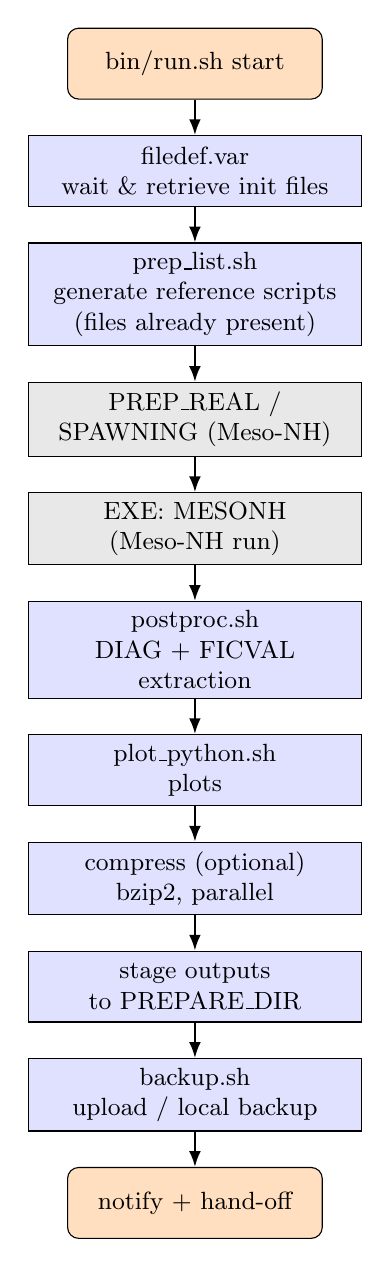
\begin{tikzpicture}[node distance=0.45cm]
\node[startstop] (start) {bin/run.sh start};
\node[process, below=of start] (filedef) {filedef.var\\wait \& retrieve init files};
\node[process, below=of filedef] (prep) {prep\_list.sh\\generate reference scripts\\(files already present)};
\node[mesonh, below=of prep] (real) {PREP\_REAL / SPAWNING (Meso-NH)};
\node[mesonh, below=of real] (exe) {EXE: MESONH (Meso-NH run)};
\node[process, below=of exe] (postproc) {postproc.sh\\DIAG + FICVAL extraction};
\node[process, below=of postproc] (plot) {plot\_python.sh\\plots};
\node[process, below=of plot] (compress) {compress (optional)\\bzip2, parallel};
\node[process, below=of compress] (stage) {stage outputs\\to PREPARE\_DIR};
\node[process, below=of stage] (backup) {backup.sh\\upload / local backup};
\node[startstop, below=of backup] (notify) {notify + hand-off};
\draw[wkarrow] (start) -- (filedef);
\draw[wkarrow] (filedef) -- (prep);
\draw[wkarrow] (prep) -- (real);
\draw[wkarrow] (real) -- (exe);
\draw[wkarrow] (exe) -- (postproc);
\draw[wkarrow] (postproc) -- (plot);
\draw[wkarrow] (plot) -- (compress);
\draw[wkarrow] (compress) -- (stage);
\draw[wkarrow] (stage) -- (backup);
\draw[wkarrow] (backup) -- (notify);
\end{tikzpicture}
\caption{Internal phase sequence of \texttt{bin/run.sh}. Grey boxes are Meso-NH itself; blue boxes are
automation scripts.}
\label{fig:runsh}
\end{figure}

Each of these phases can be individually disabled for debugging via the \texttt{NOPREP}\slash
\texttt{NORUN}\slash\texttt{NODIAG}\slash\texttt{NOFICVAL}\slash\texttt{NOPLOT} switches in
\texttt{globals.var}; this is intended for manual troubleshooting only.

\texttt{bin/pgdgen.sh} is a separate, standalone script (not called by \texttt{run.sh}) used to
(re-)generate the static PGD orography files for a site; it is normally run once, at installation time
(Section~\ref{sec:deps-install}), and only re-run if the domain geometry or the ground/topography input
files change.

The scripts \texttt{bin/Run\_lista.sh}, \texttt{bin/crossc2d.py} and \texttt{bin/multi.py} are
CPU/timing benchmarking helpers used to test the code against a list of past initialization dates; they
are not part of the nightly operational workflow.

\subsection{Directory layout}
The automation lives in one top-level working directory (\texttt{WORKDIR} in \texttt{globals.var}):
\begin{lstlisting}
bin/            : scripts (see Section 5)
bin/conf.d/     : configuration files, namelist templates, correction tables, compiled
                   fortran helpers (see Section 4)
PGD/            : static orography files, generated once by pgdgen.sh and persistent
                   across runs
\end{lstlisting}
The following sub-directories are created fresh by each run and removed/replaced at the end of it
(anything left behind after a failed run is there for post-mortem debugging only, and will be deleted
on the next successful run):
\begin{lstlisting}
REAL/     : PREP_REAL binary output and namelists
RUN/      : Meso-NH (EXE) binary output and namelists
DIAG/     : DIAG / conv2dia binary output and namelists
ASCII/    : ASCII output of the postprocessing (DAT, FICVAL, PLOT_DAT, AUTOREGRESSION
            sub-directories)
PLOT/     : figures produced by the Python plotting suite
LOG/      : logs of the current/last run
\end{lstlisting}
Outside \texttt{WORKDIR}, in the automation user's home directory, the following are used across runs:
\begin{lstlisting}
<init dir>/          : combined (orography + forecast) init files for the current night
                        (INIDIR)
<backup init cache>/ : local cache of files retrieved from the backup init server
                        (BKSERVER_LOCALPATH)
BACKUP_OUTPUT/        : per-night backup of ASCII/plot outputs (see backup.var)
BACKUP_FIGURES/        : local mirror of the delivered figures
<staging dir>/         : staging directory used while moving outputs (PREPARE_DIR)
AUTOREGRESSION/         : hand-off area shared with the short-timescale component,
                          if in use on this deployment
TOPOGRAPHY/             : source topography files used to build the PGD
<python virtualenv>/   : Python virtualenv used by the automation (Section 3)
\end{lstlisting}
The exact names in angle brackets above are whatever \texttt{globals.var} currently sets them to
(Section~\ref{sec:config}); they are not fixed by the code.

\subsection{Logging and alerting}
Each phase writes to its own timestamped log file under \texttt{LOGDIR} (main log, error log, and one
log per Meso-NH executable), configured in \texttt{globals.var}. A cumulative log recording start/end
time and duration of every phase of every run is appended to the path set by
\texttt{LOG\_TIME\_CUMULATIVE} in \texttt{globals.var}. Fatal problems abort the script and send an
alert e-mail (function \texttt{error}); non-fatal issues are logged and mailed without stopping the run
(function \texttt{error\_soft}).

\section{DEPENDENCIES AND INSTALLATION}
\label{sec:deps-install}

\subsection{Assumed pre-requisites}
This section assumes that \textbf{Meso-NH} and a matching local \textbf{OpenMPI} build are already
installed and working. The codebase currently in use expects Meso-NH \textbf{V5.2.1} built against
\textbf{eccodes 2.30.0}, set in \texttt{globals.var} as:
\begin{lstlisting}
MNH_BASE_PATH="${HOME}/MNH-V5-2-1_eccodes_2_30_0"
\end{lstlisting}
and OpenMPI \textbf{4.1.1}. A custom Meso-NH \texttt{VER\_USER} build is required; which build is active
is selected by \texttt{MESONH\_PERSO\_VERSION} in \texttt{globals.var} (Section~\ref{sec:config}). On
this deployment it switches seasonally (winter/summer) between two builds, because the optical-
turbulence calibration built into the model is itself seasonal and the switch is driven by the current
date; a fixed, non-seasonal build can also be used (see the note in Section~\ref{sec:config}).

\textbf{A note on Meso-NH output format.} This codebase reads and writes Meso-NH's legacy \texttt{.lfi}
binary output format throughout (PREP\_REAL, EXE and DIAG outputs, the optional \texttt{bzip2}
compression step, the \texttt{conv2dia}/\texttt{diaprog} post-processing). It has \textbf{not} been
adapted to the \texttt{.nc4}/NetCDF-4 output format used by more recent Meso-NH versions; deploying it
against a Meso-NH build that only produces \texttt{.nc4} output will require changes to the
post-processing chain that are outside the scope of this manual.

\subsection{System-level dependencies}
\begin{table}[H]
\centering
\begin{tabular}{|l|l|}
\hline
\textbf{PROGRAM} & \textbf{NOTES} \\ \hline
Meso-NH & V5.2.1, custom VER\_USER build (see above) \\
OpenMPI & 4.1.1 \\
eccodes (incl.\ \texttt{grib\_copy}) & 2.30.0, used to merge orography into forecast grib files \\
gfortran + \texttt{make} & used to build the helper programs in \texttt{bin/conf.d/utils} \\
bash & \(\geq\)4.x \\
Python 3 & used both directly and inside a dedicated virtualenv (below) \\
GNU \texttt{parallel} & parallel \texttt{bzip2} compression of Meso-NH output \\
ImageMagick (\texttt{convert}) & format conversion in the plotting phase \\
\texttt{bc} & floating point arithmetic in the bash scripts \\
OpenSSH client (\texttt{ssh}\slash\texttt{scp}) & retrieval from the backup init server, uploads \\
\texttt{rsync} & delivery of figures/ASCII outputs and hand-off to the AR hosts \\
\hline
\end{tabular}
\end{table}

\subsection{Python environment}
The automation code expects a Python virtualenv at a fixed path referenced by \texttt{LOCPYTHONDIR} in
\texttt{globals.var}; \texttt{run.sh} activates it at the start of every run and deactivates it at the
end. If a short-timescale component is also installed on the same host, it can share this same
virtualenv.

The packages required by the automation scripts themselves (plotting, ephemerides, mail) are:
\begin{lstlisting}
numpy
scipy
matplotlib
pytz
python-dateutil
ephem
google-api-python-client
google-auth
\end{lstlisting}
If the same virtualenv is also used to run a short-timescale/AR component, check that component's own
environment manual for any additional version constraints; they are not needed by the automation code
on its own.

To create the environment from scratch:
\begin{lstlisting}
cd $HOME
python3 -m venv <venv_name>
source $HOME/<venv_name>/bin/activate
pip install --upgrade pip
pip install numpy scipy matplotlib pytz python-dateutil ephem \
            google-api-python-client google-auth
deactivate
\end{lstlisting}
(replace \texttt{<venv\_name>} with whatever \texttt{LOCPYTHONDIR} in \texttt{globals.var} points at).

\subsection{Mail delivery (Gmail API)}
Alert and completion e-mails are sent through the Gmail API rather than through a local MTA, via
\texttt{sendmail\_gmail.py} under \texttt{bin/conf.d/utils/} -- this is the script actually wired into
every alert path, through \texttt{common\_functions.func}. It expects an OAuth client secret and a
cached token in the Python virtualenv directory:
\begin{lstlisting}
<venv_name>/credentials.json   : OAuth 2.0 client secret (download from the Google Cloud
                                  project used for this mail account)
<venv_name>/token.pickle       : cached, auto-refreshed OAuth token; generated on first
                                  successful authentication
\end{lstlisting}
A same-named \texttt{sendmail\_attach.py} also exists under \texttt{bin/conf.d/utils}, using a plain
\texttt{smtplib}\slash SMTP implementation instead, but it is not currently invoked anywhere in this
codebase; it can be ignored for installation purposes.
Setting up \texttt{credentials.json} and performing the first interactive authorization (to create
\texttt{token.pickle}) must be done once, outside of the automated procedure, before the first scheduled
run; afterwards the token is refreshed automatically. Without valid credentials the scripts abort rather
than silently failing to notify.

\subsection{Installation steps}
\begin{enumerate}
  \item \textbf{Unpack the code.} Extract the automation directory to its intended location (it can
        live anywhere, but conventionally directly under the automation user's home directory).
  \item \textbf{Point the configuration at its working directory.} In
        \texttt{bin/conf.d/globals.var}, set \texttt{WORKDIR} to the absolute path of that directory.
  \item \textbf{Build the fortran helper programs.} These are not portable binaries and must be
        recompiled on the target machine:
        \begin{lstlisting}
        cd bin/conf.d/utils
        ./Make_All.sh
        \end{lstlisting}
        This builds every helper under a \texttt{source\_*} sub-directory (post-processing and
        correction tools used by \texttt{postproc.sh}\slash\texttt{plot\_python.sh}); the script aborts
        on the first compilation failure, so a clean run confirms the whole helper suite is usable.
  \item \textbf{Set up the Python virtualenv and the Gmail API credentials} as described above.
  \item \textbf{Set up passwordless SSH (key-based)} from the automation account to three groups of
        remote hosts. First, the backup initialization server
        (\texttt{BKSERVER\_USER}\slash\texttt{BKSERVER\_IP} in \texttt{globals.var}). Second, the
        primary and backup output servers (\texttt{REMOTE\_USER}\slash\texttt{REMOTE\_HOST} and
        \texttt{REMOTE\_USER\_BK}\slash\texttt{REMOTE\_HOST\_BK}, both in \texttt{backup.var}). Third,
        if a short-timescale component is deployed, its hand-off host(s)
        (\texttt{REMOTE\_AR}\slash\texttt{REMOTE\_AR\_BK}, also in \texttt{backup.var}).
  \item \textbf{Generate the PGD (orography) files.} Once the topography source files are in place
        (\texttt{TOPODIR} in \texttt{globals.var}) and \texttt{pgd.var} is configured for the site
        (Section~\ref{sec:config}):
        \begin{lstlisting}
        cd bin
        ./pgdgen.sh
        \end{lstlisting}
        A successful run populates \texttt{PGD/}. This step only needs to be repeated if the domain
        geometry, nesting configuration or ground/topography input files change; it is otherwise a
        one-time step per site.
  \item \textbf{Do a manual test run} before relying on cron:
        \begin{lstlisting}
        cd bin
        ./run.sh
        \end{lstlisting}
        Inspect \texttt{LOG/} for errors; the most common causes of failure at this stage are a
        missing/incorrect \texttt{WORKDIR}, missing PGD files, an un-built helper program, or missing
        SSH/API credentials.
  \item \textbf{Install the cron entry} shown in Section~\ref{sec:usage} for nightly operation.
\end{enumerate}

\section{CONFIGURATION}
\label{sec:config}

\subsection{Main files}
Inside the working directory tree, the executables and configuration files that a user is expected to
interact with are the following:
\begin{table}[H]
\centering
\begin{tabular}{llll}
\hline
\multirow{7}{*}{bin/}\hspace{1.2cm}\ldelim\{{7}{10pt} & run.sh & :main nightly executable\\
 & pgdgen.sh & :one-time PGD (orography) generation\\
 & prep\_list.sh & :generates reference legacy-style scripts, called by run.sh\\
 & postproc.sh & :DIAG/FICVAL extraction, sourced by run.sh\\
 & backup.sh & :upload/backup, sourced by run.sh\\
 & plot\_python.sh & :plotting, sourced by run.sh\\
 & Run\_lista.sh & :Run in postprocessing on a sequence of dates\\
\multirow{6}{*}{bin/conf.d/}\ldelim\{{6}{10pt} & globals.var & :main configuration file (paths, logging, MNH/MPI setup)\\
 & pgd.var & :orography/PGD generation configuration\\
 & run.var & :simulation, spatial and DIAG/plot extraction parameters\\
 & times.var & :date, time and plot-window configuration\\
 & filedef.var & :init file naming/retrieval logic (mostly scripted)\\
 & backup.var & :upload and backup configuration\\
\hline
\end{tabular}
\end{table}
Other files under \texttt{bin/} and \texttt{bin/conf.d/} not listed here (and not described in
Section~\ref{sec:executables}) are internal helpers, legacy variants or testing scripts; they should
not normally need to be touched.

Further sub-directories of \texttt{bin/conf.d/} are used as follows:
\begin{lstlisting}
bin/conf.d/namelist/cen4th/   : Meso-NH namelist templates actually used by this
                                 configuration (centred 4th-order advection scheme;
                                 referenced by NLDIR in globals.var)
bin/conf.d/namelist/weno3/    : an alternative (WENO 3rd-order advection scheme)
                                 namelist set, physically present but not referenced
                                 by any current .var file -- a leftover from a
                                 different configuration this code was derived from
\end{lstlisting}
Most Meso-NH namelist parameters are set from \texttt{run.var}/\texttt{times.var} at run time; the
namelist templates only need to be edited directly for parameters that are not exposed as \texttt{.var}
variables. This should only be done by someone familiar with Meso-NH namelists.\\
\textbf{NOTE CAREFULLY:} namelist templates are edited through keyword substitution. All strings that end with \texttt{\_VALUE} or \texttt{\_FILE} are typically edited automatically. Do not change them if you do not want to make automatic substitution to silently fail.\\

\begin{lstlisting}
bin/conf.d/corrections/       : per-parameter multiplicative/additive calibration tables,
                                 applied during postprocessing (plot_python.sh)
\end{lstlisting}
Each file is a small ASCII table: one line of \texttt{MULT SUM}, or of \texttt{MULT SUM START END} for
time-windowed corrections. Files are named after the parameter they calibrate (e.g.\
\texttt{pwv\_integ.var}, \texttt{tau\_integ.var}), with some parameters also carrying seasonal variants.
Several parameters have both a default
table and an \texttt{\_OS18} variant; both are actively used by \texttt{plot\_python.sh} to compute an
alternative (``OS18'') product -- for seeing, isoplanatic angle and coherence time -- alongside the
default one; see the note on \texttt{plot\_python.sh} in Section~\ref{sec:executables}.
\begin{lstlisting}
bin/conf.d/utils/              : compiled fortran helper programs and their sources
                                  (source_* sub-directories, built by Make_All.sh, see
                                  Section 3), the Python plotting suite (Plot_python/),
                                  the Gmail-API mail senders, small ephemeris helpers
                                  (Sunset.py, Sunrise.py, Dawn.py, Dusk.py) and
                                  common_functions.func (the bash functions -- log,
                                  error, error_soft, check_directory, etc. -- sourced by
                                  every script in bin/)
\end{lstlisting}

\subsection{How to read the parameter tables below}
For each configuration file, parameters are listed with a short description and their current value,
shown as \texttt{[current: ...]} -- i.e.\ whatever this particular installation's configuration files
happen to contain today, given purely as a worked example of the kind of value expected, not as a
recommended or universal default. A variable not documented below is either a purely internal/scripted
variable (computed from other variables, not meant to be edited), a debug switch, or an
undocumented/experimental feature -- such variables should only be changed by someone who has read the
corresponding script.

\subsection{globals.var}
\texttt{globals.var} holds the global configuration: debug switches, the Meso-NH/MPI/Python setup, the
main working paths, logging and the init/output path tree. It is sourced first by every script.

\subsubsection{Debug switches}
\begin{lstlisting}
TESTRUN=0/1        : if 1, do not wait for real init files; use whatever init files are
                      manually specified/present instead. See section~\ref{sec:filedef} to understand how it works. [current: 0]
PREPLISTTRUE=0/1   : if 1, run.sh invokes prep_list.sh at the start of the run. [current: 1]
WAITSURE=0/1       : if 1, wait one extra minute after all init files are detected, to be
                      extra sure the upload has really finished. [current: 0]
PARSEBACKUP=0/1    : internal use only, must be left at 0.
BACKUPLATER=0/1    : if 1, backup.sh is not sourced automatically at the end of run.sh
                      (it must then be run separately by hand or by an external wrapper
                      script, which this codebase does not provide). [current: 0]
NOPREP/NORUN/
NODIAG/NOFICVAL/
NOPLOT=0/1         : debug switches to individually skip the PREP_REAL, EXE, DIAG,
                      FICVAL-extraction or PLOT phase. All [current: 0]; only meant for
                      manual troubleshooting (see the workflow description above).
\end{lstlisting}

\subsubsection{Meso-NH / MPI version}
\begin{lstlisting}
SHORTVERSION="string"        : short tag for the Meso-NH version, used in log/output file
                                names. [current: "M521"]
MNH_BASE_PATH="string"       : root of the Meso-NH installation.
                                [current: "${HOME}/MNH-V5-2-1_eccodes_2_30_0"]
MESONH_PERSO_VERSION="string": name of the custom Meso-NH VER_USER build to use. On this
                                deployment it is computed automatically from the current
                                month (a "winter" build for Oct-Mar, a "summer" build for
                                Apr-Sep), each hard-coded as a commented-out fallback just
                                above the seasonal if/else, so a fixed build can be forced
                                by uncommenting one and removing the seasonal logic. The
                                winter/summer split is a seasonal calibration of the
                                optical-turbulence model built into that version, not a
                                change of advection scheme -- see Section 3.1.
MPI_VERSION="string"         : root of the local OpenMPI installation.
                                [current: "${HOME}/OPEN-MPI-4-1-1"]
\end{lstlisting}
\texttt{MNH\_MAIN\_PATH}, \texttt{MNH\_GRIBAPI\_PATH}, \texttt{MNH\_TOOL\_PATH}, \texttt{MNH\_PROFILE}
and the \texttt{LD\_LIBRARY\_PATH}\slash\texttt{PATH} exports below them are derived automatically from
the three variables above and from Meso-NH's own \texttt{profile\_mesonh}; they should only need to
change together with a Meso-NH/eccodes version upgrade.

\subsubsection{Base configuration and main paths}
\begin{lstlisting}
SITE_NAME="string"  : max 3 characters, identifies the site. [current: 3-letter site tag]
NESTING=integer     : number of nested domains (outer=1). [current: 3]
WORKDIR="string"    : absolute path of the automation's working directory. Must be
                      edited at install time (see the Installation steps above).
LOCPYTHONDIR="string": bin/ directory of the Python virtualenv activated by run.sh.
PYTHONEXE="string"  : Python interpreter name. [current: "python3"]
\end{lstlisting}
\texttt{CONFDIR}, \texttt{EXEDIR}, \texttt{UTILDIR}, \texttt{PYTHONPLOT}, \texttt{FUNCFILE} and the
\texttt{*\_VAR} variables pointing at the other configuration files (\texttt{FILEDEF\_VAR},
\texttt{TIME\_VAR}, \texttt{TIME\_VAR\_SEQ}, \texttt{RUN\_VAR}, \texttt{PGD\_VAR},
\texttt{BACKUP\_VAR}, \texttt{CORRECTION\_DIR}) are all derived from \texttt{WORKDIR} and should not
normally be edited.

\subsubsection{Logging}
\begin{lstlisting}
LOGEXE=0/1/2      : 0 prints MESONH output to the console; 1 sends it to separate log
                    files; 2 appends it to the main log file. [current: 1]
MAIL_ADDRESS="string": destination address(es) for alert/completion mail.
FROM_ADDRESS="string": sender address used by the Gmail-API mail scripts.
MAIL_PREFIX="string" : subject-line prefix for all mail from this deployment. Built as
                    "<project tag> - ${NESTING}DOM"; the checked-in value still carries a
                    project tag inherited from the codebase this automation was derived
                    from -- edit it to identify your own deployment.
\end{lstlisting}
\texttt{LOGDIR} and every \texttt{LOG*FILE} variable are timestamped paths derived from
\texttt{WORKDIR}/\texttt{DATESTART}; \texttt{LOG\_TIME\_CUMULATIVE} and \texttt{ERROR\_OUTPUT\_FILE}
live outside \texttt{WORKDIR}, directly under \texttt{\$HOME}, so that they survive across runs (the
cumulative timing log and the hard-error marker file, respectively). \textbf{Note:} the comment
immediately above \texttt{ERROR\_OUTPUT\_FILE} in the checked-in file still warns to also update an
external orchestration script if this variable is renamed; that script is not part of this codebase (see
the note on scope in Section~\ref{sec:usage}) and the comment is stale -- safe to ignore, or to remove,
on this single-configuration deployment.

\subsubsection{Init paths}
\begin{lstlisting}
INIRAWDIR="string"       : directory where raw initialization files are uploaded by the
                           forecast-model data provider.
INIDIR="string"          : directory where the merged (orography+forecast) files are
                           placed, by the retrieval logic in filedef.var.
BKSERVER_USER="string"   : SSH username on the backup init server. Requires
                           passwordless key-based login (see the Installation steps).
BKSERVER_IP="string"     : IP of the backup init server.
BKSERVER_INIPATH="string": remote path (relative) of the init files on that server.
BKSERVER_LOCALPATH="string": local cache directory for files retrieved from it.
\end{lstlisting}

\subsubsection{Output paths}
The remaining paths in this block are almost all mechanically derived from \texttt{WORKDIR} or
\texttt{\$HOME} and are not normally edited by hand; they are listed here for completeness since they
determine where each phase's output can be found (Section~\ref{sec:usage}, ``Directory layout''):
\begin{table}[H]
\centering
\begin{tabular}{|p{4.8cm}|p{10cm}|}
\hline
\textbf{Variable} & \textbf{Purpose} \\ \hline
OUTDIR\_REAL / OUTDIR\_PREP & PREP\_REAL binary output and namelists (\texttt{WORKDIR/REAL}) \\ \hline
OUTPUT\_MNH / PREP\_MNH & EXE (Meso-NH run) binary output and namelists (\texttt{WORKDIR/RUN}) \\ \hline
DIAG\_MNH / PREP\_DIAG & DIAG/conv2dia binary output and namelists (\texttt{WORKDIR/DIAG}) \\ \hline
ASCII\_DIR, DAT\_DIR, PLOTDAT\_DIR, FICVAL\_DIR & ASCII postprocessing output (\texttt{WORKDIR/ASCII/...}) \\ \hline
AUTOREGRESSION\_DIR & per-run ASCII staged for the short-timescale hand-off (\texttt{ASCII\_DIR/AUTOREGRESSION}) \\ \hline
PLOT\_DIR & figures produced by the plotting phase (\texttt{WORKDIR/PLOT}) \\ \hline
AUTOREGRESSION\_-\newline STORE\_DIR & final hand-off data store, a site-named
 subdirectory under \texttt{\$HOME/AUTOREGRESSION} \\ \hline
AUTOREGRESSION\_-\newline BASE\_DIR & hand-off root, rsynced to the short-timescale host(s) (\texttt{\$HOME/AUTOREGRESSION}) \\ \hline
TRENDSDIR & trend files (\texttt{\$HOME/TRENDS}) \\ \hline
FINALOUTDIR & final ground-parameter output file, delivered to the telescope infrastructure;
 path under \texttt{\$HOME} is deployment-specific \\ \hline
PREPARE\_DIR & per-run staging directory before backup/upload; path under \texttt{\$HOME}
 is deployment-specific \\ \hline
PGDDIR / PREP\_PGDDIR & PGD files (\texttt{WORKDIR/PGD}) \\ \hline
TOPODIR & source topography files (\texttt{\$HOME/TOPOGRAPHY}) \\ \hline
FILTERDIR & short-timescale-component working files (\texttt{\$HOME/FILTER}) \\ \hline
\end{tabular}
\end{table}
As with \texttt{MAIL\_PREFIX} above, several of these paths still carry, in the checked-in file, naming
inherited from the codebase's origin -- among them \texttt{INIDIR}, \texttt{LOCPYTHONDIR}, the
autoregression store path, \texttt{FINALOUTDIR}, \texttt{PREPARE\_DIR}, and the backup-server and
raw-init-directory variables above. Rename them freely to fit your own deployment; nothing else depends
on the literal strings, only on the variables pointing at consistent, existing directories.

\subsubsection{Namelist templates and executables}
\texttt{NLDIR} and the \texttt{NL*} variables point at the namelist template files under
\texttt{bin/conf.d/namelist/} (Section~4.1); on this deployment \texttt{NLDIR} points at the
\texttt{cen4th} set. The \texttt{EXE\_*}/\texttt{GRIBCOPY} variables are the paths to the Meso-NH
executables and to \texttt{grib\_copy}, derived from the Meso-NH paths above; they should not need
manual editing on a standard installation.

\subsubsection{File compression and backup}
\begin{lstlisting}
DOZIPREAL=0/1  : bzip2-compress the PREP_REAL .lfi output. [current: 0]
DOZIPOUT=0/1   : bzip2-compress the EXE (Meso-NH run) .lfi output. [current: 0]
DOZIPDIAG=0/1  : bzip2-compress the DIAG .lfi output. [current: 0]
\end{lstlisting}

\subsection{pgd.var}
\texttt{pgd.var} configures the generation of the static PGD (orography) files by \texttt{pgdgen.sh}
(Section~\ref{sec:deps-install}). On this deployment it describes a domain hierarchy of up to 4 nested
levels, even though \texttt{NESTING} (in \texttt{globals.var}) is currently 3: it is \texttt{NESTING}
that determines how many of those levels \texttt{pgdgen.sh} actually generates, so the file can safely
carry parameters for one more level than is presently used, ready for a future domain to be enabled.

\begin{lstlisting}
PGDEXTRACTPT=0/1  : extract latitude/longitude/altitude from the PGD files (only useful
                    if NESTING>1). [current: 1]
PGD_PREFIX="string": 3-character site prefix for generated file names.
                    [current: "${SITE_NAME}"]
XRPK_VALUE=real   : projection type: 0=Mercator, 1=north polar, -1=south polar (write as
                    a real number, e.g. "1." not "1"). [current: "0."]
YCOVER_FILE="string": ground cover file (no extension). [current: "ECOCLIMAP_II_EUROP_V2.3"]
YCLAY_FILE="string" : clay file (no extension). [current: "CLAY_HWSD_MOY"]
YSAND_FILE="string" : sand file (no extension). [current: "SAND_HWSD_MOY"]
XLATCEN_VALUE=real  : latitude of the domain centre (site-specific).
XLONCEN_VALUE=real  : longitude of the domain centre (site-specific).
NIMAX_VALUE=integer : outer-domain grid points along X. [current: "80"]
NJMAX_VALUE=integer : outer-domain grid points along Y. [current: "${NIMAX_VALUE}"]
XDX_VALUE=meters     : outer-domain grid spacing along X. [current: "10000"]
XDY_VALUE=meters     : outer-domain grid spacing along Y. [current: "${XDX_VALUE}"]
\end{lstlisting}

The following are bash arrays. \texttt{YZS\_FILE}/\texttt{YFILETYPE\_VALUE} have one element per
domain \emph{including} the outer one (element \texttt{0} = outer domain, element \texttt{1} = first
nested domain, and so on); the other four arrays below have one element per \emph{nested} domain only,
since the outer domain has no parent to be positioned/scaled against (element \texttt{0} = first
nested domain, i.e.\ the second domain overall, element \texttt{1} = second nested domain, and so on):
\begin{lstlisting}
YZS_FILE[n]="string"        : topography source file (no extension) for domain n+1 (n=0
                               is the outer domain). Global coverage datasets (e.g.
                               "gtopo30") are typically used for the outer levels, and a
                               finer, site-specific high-resolution dataset for the
                               innermost nested level(s) -- named after the site on this
                               deployment.
YFILETYPE_VALUE[n]="string" : Meso-NH file-type keyword matching YZS_FILE[n] (e.g. DIRECT,
                               LATLON). [current: "DIRECT" for all domains]
IXOR_PREC[n], IYOR_PREC[n]  : starting grid point (X,Y) of nested domain n+2, expressed on
                               its parent (preceding) domain grid.
IXSIZE_VALUE[n],
IYSIZE_VALUE[n]             : number of grid points of nested domain n+2.
IDXRATIO_VALUE[n],
IDYRATIO_VALUE[n]           : grid-refinement ratio of nested domain n+2 with respect to
                               its parent domain.
\end{lstlisting}
These last four arrays only need to change if the domain geometry itself changes (position, extent or
resolution of a nested domain); doing so requires re-running \texttt{pgdgen.sh}.

\subsection{run.var}
\texttt{run.var} holds the Meso-NH simulation parameters proper (timestep, nesting, microphysics,
domain geometry), the plotting height/limit parameters, and the configuration of the DIAG/FICVAL
extraction (which parameters, at which points/domains/heights, are exported as ASCII for plotting and
for the short-timescale hand-off). Most variable names mirror the corresponding Meso-NH namelist
keyword. This file must be sourced after \texttt{times.var}.

\subsubsection{Simulation parameters}
\begin{lstlisting}
NUM_PROC=integer   : number of MPI processes for the simulation. [current: 64]
NAM_SIMU="string"  : 5-character CEXP (Meso-NH experiment name). [current: "${DAY}_${MONTH}"]
NAM_SEG="string"   : 5-character CSEG (Meso-NH segment name). [current: "y${YEAR}"]
NMODEL_VAR=integer : number of models/domains, normally equal to NESTING.
XTSTEP_VAR=seconds : outermost-domain Meso-NH timestep. [current: 12]
NDTRATIO_ARRAY[n]  : timestep ratio of nested level n+1 with respect to its parent
                     (element [0]=1 always). [current: 1,2,3,4]
NDAD_ARRAY[n]      : parent-level index of nested level n+1 (element [0]=1 always).
                     [current: 1,1,2,3]
XRIMKMAX[n]        : maximum lateral-relaxation coefficient (1/s) for nested level
                     n+1; kept hand-tuned rather than auto-computed (a commented-out
                     auto-generation formula is kept in the file for reference, but is
                     not used -- it was found to lead to instability).
                     [current: 0.0006666, 0.0020000, 0.0013333]
CCLOUD_VAR="string": microphysical scheme. [current: "KESS"]
CPRESOPT_VALUE="string": pressure solver. [current: "ZRESI"]
NUMOUTTIMES=integer: number of Meso-NH (.lfi) output times. [current: 15]
OUTTIMESTEP=seconds: interval between outputs; defaults to EXITSEC from times.var --
                     changing one without the other causes inconsistencies.
\end{lstlisting}
\texttt{XSEGLEN} (total simulated seconds) and the \texttt{XFMOUT[]} array (the list of output times
themselves) are computed automatically from \texttt{NUMOUTTIMES} and \texttt{OUTTIMESTEP}; they should
not be edited directly.

\subsubsection{Spatial configuration and coordinates}
\begin{lstlisting}
XSNG1="string", YSNG1="string": grid coordinates (I,J) of the first extraction point
                     (p1.dat). [current: "61","61"]
XSNG2="string", YSNG2="string": grid coordinates (I,J) of the second extraction point
                     (p2.dat). [current: "60","61"]
SEESTPOINT="string" : starting point index for seeing integration (see_p1_v.dat).
                     [current: "2"]
DOM_FIRST="string"  : nesting level of the first extraction point (1=outer). [current: "3"]
DOM_SECOND="string" : nesting level of the second extraction point. [current: "3"]
SUPCOMP_VAR="F"     : enables supplementary computations; always "F" in operation.
MESODIAG_VAR="F"    : "F"=normal run, "T"=DIAG-only mode (internal use).
NKMAX_VALUE="string": number of vertical levels. [current: "54"]
ZDZGRD_VALUE="string": near-ground vertical mesh size (m). [current: "20"]
ZDZTOP_VALUE="string": near-top vertical mesh size (m). [current: "600"]
ZZMAX_STRGRD_VALUE="string": altitude (m) separating the two constant-stretching layers.
                     [current: "3500"]
ZSTRGRD_VALUE="string": constant stretching (%) in the lower layer. [current: "20"]
ZSTRTOP_VALUE="string": constant stretching (%) in the upper layer. [current: "00"]
\end{lstlisting}

\subsubsection{Plot parameters}
\begin{lstlisting}
PLOTBASEH1, PLOTBASEH2 : lower plot height limits (m). [current: 20, 600]
PLOTTOPH1, PLOTTOPH2   : upper plot height limits (m). [current: 600, 20000]
CN2H2=meters           : intermediate height limit for CN2/wind/RH plots. [current: 2000]
MRH2=meters            : intermediate height limit for mixing-ratio plots. [current: 5000]
CN2_WRESCALE_H=meters  : height above which the wind-gradient correction is applied to
                          CN2 profiles. [current: 700]
CN2_ALPHA, CN2_BETA    : coefficients of that correction. [current: 1., 1.5]
DOM_FIRST_DX,
DOM_SECOND_DX=km       : grid spacing used for 2D maps (must match the PGD grid).
                          [current: 0.5, 0.5]
WINDSPEEDHIGHLIM=m/s   : threshold on the average near-ground (K=4) wind speed, above
                          which backup.sh still uploads the wind figures/maps even when
                          full-figure upload is otherwise disabled -- see
                          Section~\ref{sec:usage}. [current: 8.5]
\end{lstlisting}
Changes to this block generally require matching manual edits to \texttt{plot\_python.sh}.

\subsubsection{DIAG/FICVAL extraction parameters}
These control which parameters are exported by the DIAG/FICVAL phase (\texttt{postproc.sh}), and are
also the parameters whose file layout \texttt{plot\_python.sh} depends on -- changing them may require
matching edits there.
\begin{lstlisting}
EXTRACTLIST_DOM_FIRST,
EXTRACTLIST_DOM_SECOND="string": space-separated list of diaprog keywords for 2D ground
                     maps / point extraction, for DOM_FIRST and DOM_SECOND respectively.
                     [current: DOM_FIRST carries the full list (wind, SNG, SCI, ISO, CHT,
                      ECH and 200/10227/9276/6677 m wind levels), DOM_SECOND empty]
EXTRACTLIST_MULTIHEIGHT="string": keywords extracted as a function of height.
                     [current: "SNG_STAR_SUP CHT_STAR_SUP"]
PVLIST_DOM_FIRST,
PVLIST_DOM_SECOND="string": diaprog keywords for vertical profile extraction.
                     [current: both empty]
STARTPV_I[0],STARTPV_J[0]: grid point for the DOM_FIRST-related vertical profile.
                     [current: 61,61]
STARTPV_I[1],STARTPV_J[1]: grid point for the DOM_SECOND-related vertical profile.
                     [current: 51,51]
CVLIST_DOM_FIRST,
CVLIST_DOM_SECOND="string": diaprog keywords for vertical cuts. [current: both empty]
STARTCV_I/J[0], ENDCV_I/J[0]: start/end grid points of the DOM_FIRST-related vertical
                     cut. [current: (2,61) to (121,61)]
STARTCV_I/J[1], ENDCV_I/J[1]: start/end grid points of the DOM_SECOND-related vertical
                     cut. [current: (2,51) to (101,51)]
NUMLEVELDIAG=integer: number of nesting levels on which DIAG runs. [current: 1]
DIAGLEVELARRAY[n]   : which nesting level DIAG runs on, for each of the NUMLEVELDIAG
                     entries. [current: [0]=$DOM_FIRST, [1]=$DOM_SECOND (only [0] used
                     since NUMLEVELDIAG=1)]
DIAGINFHEIGHTS[n],
DIAGSUPHEIGHTS[n]   : space-separated lists of lower/upper integration heights for
                     DIAGLEVELARRAY[n]; every INF-SUP combination is computed.
                     [current: [0]="$PLOTBASEH1 $PLOTBASEH2" / "$PLOTTOPH1 $PLOTTOPH2"]
DOMP1=1, DOMP2=2    : fixed identifiers for the two extraction-point domains; used
                     elsewhere in plot.sh's domain selection logic and should not be
                     changed.
\end{lstlisting}

\subsection{times.var}
\texttt{times.var} configures the date being processed, ephemerides-related timing and the plot time
window. A large part of the file (ephemerides, seasonal plot-limit computation) is scripted and should
not be edited directly.

\textbf{How the date is actually set.} At the top of the file, \texttt{YEAR}/\texttt{MONTH}/\texttt{DAY}
default to the system date (\texttt{\$(date +\%Y)} etc.), but the checked-in file immediately overrides
them with a hand-set date a few lines below (a leftover from the last manual/debug run). \textbf{Because
this codebase has no external process that refreshes \texttt{times.var} before each run}, whichever of
the two is active when \texttt{run.sh} sources this file is what gets used:
\begin{itemize}
  \item to process ``today'' automatically on every scheduled run, comment out (or remove) the
        hand-set override so the system-date lines take effect;
  \item to reprocess a specific past night, or to pin the date for a manual test run, edit the
        hand-set override directly.
\end{itemize}
There is a second file, \texttt{times.var\_sequential}, which is a template of \texttt{times.var} using
the placeholders \texttt{SET\_THE\_DATE\_YEAR}/\texttt{SET\_THE\_DATE\_MONTH}/\texttt{SET\_THE\_DATE\_DAY}/
\texttt{SET\_THE\_UPLOADFIGS} in place of literal values. Nothing in this codebase currently reads or
substitutes into this template -- it is not sourced by \texttt{run.sh}, and no other script in
\texttt{bin/} references it. It is a leftover from a deployment where an external, per-night wrapper
script generated \texttt{times.var} from it; on this single-configuration codebase either ignore it, or
use it as the starting point for your own such wrapper if you want one, substituting the four
placeholders and copying the result over \texttt{times.var} before invoking \texttt{run.sh}.

\subsubsection{Date and time}
\begin{lstlisting}
YEAR=yyyy, MONTH=mm, DAY=dd : date (UT) of the start of the forecast (see above for how
                     this is actually set).
FRCSTDATECOMPUTED=hh: UT hour at which the forecast used for initialization was computed.
                     [current: 12]
FORWARDFRCSTDATEPLUS=hours: how far in the future, from FRCSTDATECOMPUTED, the first
                     forecast file is valid for. [current: 12]
DATEFIGLT=0/1       : if 1, the date used to label figures is the local-time start of the
                     night; if 0, it is the UT date of the end of the night. [current: 1]
HOUR_SHIFT_PLOT=hours: shift of the plot time axis with respect to UT midnight, to align
                     with the simulation start. [current: 0]
UTOFFSET=hours      : local time offset from UT at the site. [current: -7]
HOUR_LIST="string"  : space-separated list of forcing hours; matching initialization
                     files must exist for each. [current: "00 06 12 18"]
TIMESEND=hh         : UT hour by which the init files are expected to have arrived.
                     [current: 18]
TIMELIMIT=seconds   : how long to keep waiting/retrying past TIMESEND before aborting
                     with an error. [current: 10800]
EXITSEC=seconds     : interval between Meso-NH output times; must match OUTTIMESTEP in
                     run.var. [current: 3600]
\end{lstlisting}
(\texttt{EXITMIN} is simply \texttt{EXITSEC/60}, computed automatically.)

\subsubsection{Plot parameters}
\begin{lstlisting}
PLOTSTARTT/PLOTSTARTEXIT, PLOTFIRSTT/PLOTFIRSTEXIT, PLOTSECONDT/PLOTSECONDEXIT,
PLOTENDT/PLOTENDEXIT       : default (non-seasonal) plot time window, in minutes from
                              simulation start and corresponding Meso-NH output index;
                              overwritten by the seasonal computation below when
                              SEASONSPLOT=1 (the default).
FIRSTMONTH=mm, LASTMONTH=mm: calendar months bounding "summer" for the seasonal plot
                              window. [current: 04, 09]
EMISPHERE=1/-1              : 1 for the northern hemisphere, -1 for the southern.
                              [current: 1]
SEASONSPLOT=0/1             : if 1 (default), the plot time window is computed each
                              night from sunset/sunrise/dusk/dawn (via the Sunset.py /
                              Dusk.py / Dawn.py / Sunrise.py helpers) instead of using
                              the fixed values above. [current: 1]
UPLOADFIGS=0/1              : tells backup.sh whether to upload all figures (1) or only
                              the wind-at-ground figures, and only if WINDSPEEDHIGHLIM is
                              exceeded (0) -- see Section~\ref{sec:usage}. A static
                              per-deployment setting here (there is no longer anything
                              that overrides it per run). [current: 1]
\end{lstlisting}

\subsection{backup.var}
\texttt{backup.var} configures what gets preserved/uploaded at the end of a run and where.

\subsubsection{Upload / backup switches}
\begin{lstlisting}
UPLOAD=0/1     : upload figures/ASCII outputs to the remote server(s). [current: 1]
ARUPLOAD=0/1   : rsync the AUTOREGRESSION hand-off directory to the short-timescale
                 component's host(s) at the end of run.sh, if that component is in use
                 on this deployment. [current: 1]
BACKUP=0/1     : perform the local backup of output files. [current: 1]
BACKUPFIGURES=0/1: keep a local mirror of the delivered figures. [current: 1]
\end{lstlisting}

\subsubsection{Backup parameters}
\begin{lstlisting}
TAIL_DIR="string"   : suffix appended to the per-night backup directory name. The
                      checked-in value is a short project tag inherited from this
                      codebase's origin; edit to identify your own deployment.
BACKUP_DIR="string" : root of the local ASCII/plot backup. [current: "${HOME}/BACKUP_OUTPUT"]
BACKUP_FIGURES_DIR="string": root of the local figures mirror.
                      [current: "${HOME}/BACKUP_FIGURES"]
BACKUP_REAL, BACKUP_RUN,
BACKUP_DIAG=0/1     : whether to keep, respectively, the PREP_REAL / EXE(RUN) / DIAG
                      binary output in the per-night backup (rather than discarding it).
                      [current: 0, 0, 0]
BACKUP_MNHDAT=0/1   : keep the ASCII (.dat, FICVAL, AUTOREGRESSION) postprocessing
                      output. [current: 1]
BACKUP_POSTPROC=0/1 : keep the ASCII+PLOT postprocessing output tree. [current: 1]
BACKUP_LOG=0/1      : keep the run's log directory (required for backup.sh to be able
                      to relocate its own log paths correctly at the end of the run).
                      [current: 1]
\end{lstlisting}
The corresponding \texttt{BACKUP\_*\_NAME} variables are the actual destination paths, all built from
\texttt{BACKUP\_BASE\_NAME} (itself \texttt{BACKUP\_DIR/<date><TAIL\_DIR>\_<N>DOM\_<MESONH version>});
they are not normally edited directly.

\subsubsection{Remote host parameters}
\begin{lstlisting}
DAYSTARTBEFORE=integer (negative): how many days before the forecast date the simulation
                      started; used to locate the right backup sub-directory.
                      [current: -1]
REMOTE_USER="string", REMOTE_HOST="string": account/host of the primary remote output
                      server. Placeholder values in the checked-in file -- must be
                      filled in for your own deployment.
REMOTE_USER_BK="string", REMOTE_HOST_BK="string": account/host of the redundant backup
                      remote server. Also placeholders in the checked-in file.
REMOTE_PATH_ARCHIVE="string", REMOTE_PATH_OUTPUTS_GROUND="string": upload paths on the
                      primary server for figures and ground-parameter ASCII output
                      respectively (trailing slash required). The checked-in values
                      still point at a path tree named after this codebase's origin;
                      edit to match your own server layout.
REMOTE_PATH_ARCHIVE_BK="string",
REMOTE_PATH_OUTPUTS_GROUND_BK="string": matching upload paths on the backup server.
REMOTE_AR="string", REMOTE_AR_BK="string": address(es) of the short-timescale
                      component's hand-off host(s), if that component is deployed;
                      the AUTOREGRESSION directory is rsynced there at the end of
                      run.sh. Placeholders in the checked-in file.
REMOTE_PATH_AUTOREG="string": remote path (trailing slash) for that hand-off rsync.
\end{lstlisting}

\subsection{filedef.var}
\label{sec:filedef}
\texttt{filedef.var} is mostly scripted logic rather than user-facing parameters: it implements the
search for the day's PGD files, and the wait/retrieval/validation of the initialization files described
in Section~\ref{sec:usage} (matching against \texttt{HOUR\_LIST} from \texttt{times.var}, retrying from
the backup init server after \texttt{TIMELIMIT}, verifying MD5 checksums, merging orography via
\texttt{grib\_copy}). It must be sourced after \texttt{run.var} and \texttt{times.var}, on which its
logic depends.

Despite the file's own header warning not to modify anything past a certain point, two variables here
\textbf{do sometimes legitimately need editing}, because they encode the forecast-data provider's
current naming convention for the delivered files rather than anything internal to FAST:
\begin{lstlisting}
BASEINITNAME="string" : expected base filename of the day's raw forecast files.
                        [current: "D2D${MONTH}${DAY}${FRCSTDATECOMPUTED}00"]
BASEANAFILE="string"  : expected filename of the initial analysis file (the one grib_copy
                        merges orography from). Built by repeating the BASEINITNAME
                        date/hour tokens and appending a trailing "001" segment.
                        [current starts: "D2D${MONTH}${DAY}${FRCSTDATECOMPUTED}00..."]
\end{lstlisting}
If the provider ever changes how it names the files it delivers, these two variables are the ones to
update to match; the rest of the search/retrieval logic is built on top of them and should not need to
change.

\textbf{TESTRUN=1 behaviour.} When \texttt{TESTRUN=1} (\texttt{globals.var}), all of the search/wait/
retrieval logic above is skipped outright, and every element of \texttt{FILE\_ANA\_ARRAY} (the array of
init file paths consumed by the rest of \texttt{run.sh}) is set to a non-existent placeholder
(\texttt{\$\{INIDIR\}/foo}) rather than a real file. For a \texttt{TESTRUN=1} run to actually work, the
commented-out block near the end of the file must be edited by hand:
\begin{lstlisting}
##################################################################
#EDIT THIS TO OVERWRITE GRIB FILES SELECTION FOR DEBUG PURPOSES
##################################################################
\end{lstlisting}
Uncommenting and filling in the \texttt{FILE\_ANA\_ARRAY[...]=...} lines there (a few worked examples,
commented out, are already present as a starting point) is what supplies real, existing file paths in
place of the placeholder -- this is not an optional convenience for advanced debugging, it is the only
way \texttt{TESTRUN=1} produces a working run at all.

\section{EXECUTABLES REFERENCE}
\label{sec:executables}
This section describes each script individually. Section~\ref{sec:usage} already covers how they fit
together into the nightly workflow; here the focus is on each script's own inputs, outputs and notable
behaviour.

\subsection{bin/run.sh -- main nightly executable}
Entry point of a single night's simulation; invoked with no arguments, either by cron or manually
(Section~\ref{sec:usage}). It locates its own configuration via \texttt{conf.d/globals.var}, relative to
its own path, so it must be run from within \texttt{bin/}. On start it kills any leftover Meso-NH-related
processes from a previous, possibly stuck run (\texttt{pkill} on the executable names from
\texttt{globals.var}), rotates the log directory, then runs the full phase sequence described in
Section~\ref{sec:usage} (\texttt{prep\_list.sh}, \texttt{filedef.var}, PREP\_REAL, EXE,
\texttt{postproc.sh}, \texttt{plot\_python.sh}, compression, staging, \texttt{backup.sh}, notification,
hand-off). Exit status is 0 on success; any hard failure calls the \texttt{error} function (log + alert
mail + \texttt{exit 1}). Individual phases can be disabled with the \texttt{NOPREP}\slash\texttt{NORUN}\slash
\texttt{NODIAG}\slash\texttt{NOFICVAL}\slash\texttt{NOPLOT} debug switches in \texttt{globals.var}
(Section~\ref{sec:config}).

\subsection{bin/prep\_list.sh -- generate reference legacy-style scripts}
Invoked by \texttt{run.sh} as a separate sub-process (\texttt{env bash -c}) before the PREP\_REAL phase,
unless \texttt{PREPLISTTRUE=0}. Its header comment (``script used to generate runscripts with all the
namelists inside, Lascaux\&Masciadri style'') is accurate and matches what most of the script actually
does: it generates \textbf{two self-contained, standalone bash scripts}, written into \texttt{WORKDIR}:
\begin{lstlisting}
1.PREP_EXP_REAL_<version>_<site>_<N>MOD_<date>_<levels>lev_<tail>  : reproduces the
                                                    PREP_REAL/SPAWNING step
2.PREP_EXP_RUN_<version>_<site>_<N>MOD_<date>_<levels>lev_<tail>   : reproduces the
                                                    EXE (Meso-NH run) step
\end{lstlisting}
Each is fully self-contained -- exported shell variables, the relevant namelists embedded via heredocs,
the exact \texttt{mpirun} invocation -- written in the style of the pre-FAST Lascaux \& Masciadri
Meso-NH workflow scripts. They are meant as \textbf{reference material for a user unfamiliar with FAST}
who wants to see, or manually reproduce, what happens at the plain Meso-NH level; \texttt{run.sh}'s own
PREP\_REAL/EXE phases are separate, inline implementations and do \textbf{not} use these generated
scripts at all.

Generating them requires knowing which init files are available, so \texttt{prep\_list.sh} does source
\texttt{globals.var}, \texttt{times.var}, \texttt{run.var}, \texttt{filedef.var} and \texttt{backup.var}
(with \texttt{GENERATELIST=1}, which suppresses the verbose logging those files would otherwise
produce). Because it runs in a separate shell, none of the variables it resolves survive back into \texttt{run.sh}. At the end, \texttt{prep\_list.sh} deletes the REAL/RUN staging directories it used while generating the scripts (\texttt{rm -rf}); only the two generated scripts are left behind in \texttt{WORKDIR}.

If invoked interactively (with any command-line argument) it will instead prompt for\\
\texttt{YEAR}/\texttt{MONTH}/\texttt{DAY}/\texttt{DAYB} rather than reading them from \texttt{times.var}.

\subsection{bin/postproc.sh -- DIAG/FICVAL extraction}
Sourced (not executed as a sub-process) by \texttt{run.sh} right after the EXE phase, so it shares
\texttt{run.sh}'s environment. Unless \texttt{NODIAG=1}, it loops over every Meso-NH output
(\texttt{.lfi}) file, and for each nesting level listed in \texttt{DIAGLEVELARRAY} runs the \texttt{DIAG}
executable and \texttt{conv2dia}/\texttt{diaprog} for every combination of heights in
\texttt{DIAGINFHEIGHTS}/\texttt{DIAGSUPHEIGHTS} (\texttt{run.var}, Section~\ref{sec:config}), producing
the derived astroclimatic parameters. Unless \texttt{NOFICVAL=1}, it also runs the FICVAL extraction
(vertical profiles/cuts and 2D ground maps) for the keywords configured in
\texttt{EXTRACTLIST\_DOM\_FIRST}/\texttt{EXTRACTLIST\_DOM\_SECOND}/\texttt{PVLIST\_*}/\texttt{CVLIST\_*}.\\
Output goes to \texttt{DIAG\_MNH}/\texttt{ASCII\_DIR} (Section~\ref{sec:usage}).

\subsection{bin/plot\_python.sh -- plotting}
Sourced by \texttt{run.sh} after \texttt{postproc.sh}, unless \texttt{NOPLOT=1}. Drives the Python
scripts under \texttt{bin/conf.d/utils/Plot\_python/} (Section~\ref{sec:config}) to turn the ASCII
output of \texttt{postproc.sh} into the delivered figures under \texttt{PLOT\_DIR}, and computes
\texttt{WINDAVG} (the K=4 average wind speed) and the derived \texttt{WINDAVGHIGH} flag against
\texttt{WINDSPEEDHIGHLIM} (\texttt{run.var}), used by \texttt{backup.sh} as described in
Section~\ref{sec:usage}. Uses ImageMagick's \texttt{convert} for at least one figure format conversion
step.

It computes the full parameter suite on \texttt{DOM\_FIRST}: CN2 (both a ``new-algorithm''
wind-gradient-corrected product and, in parallel, the \texttt{\_OS18} alternative product, Section~
\ref{sec:config}), seeing, isoplanatic angle and coherence time, potential and absolute temperature,
relative humidity, precipitable water vapour, plus wind at several fixed levels and vertical profiles,
and 2D ground maps for most of the above. Among the wind products, it also computes statistics over
three fixed height windows tied to specific instrument requirements at the deployment site
(script-internal suffixes \texttt{\_linc\_low}\slash\texttt{\_linc\_high}, \texttt{\_flao},
\texttt{\_argos} -- currently 30--415\,m, 5072--9127\,m, 30--20000\,m and 30--560\,m respectively); edit
the ranges and labels directly in the script if a different deployment's instruments need different
windows. It unconditionally copies its ground-parameter results (seeing/wind/temperature/RH/PWV) into
\texttt{AUTOREGRESSION\_DIR} and \texttt{AUTOREGRESSION\_STORE\_DIR}, ready for the short-timescale
hand-off described in Section~\ref{sec:usage}, if that component is deployed.

\subsection{bin/backup.sh -- upload and local backup}
Sourced by \texttt{run.sh} at the very end of a successful run, unless \texttt{BACKUPLATER=1} (in which
case it must be invoked separately). Reads \texttt{backup.var} (Section~\ref{sec:config}) to decide, per
output category, whether to rsync it to the primary and backup remote servers
(\texttt{REMOTE\_HOST}\slash\texttt{REMOTE\_HOST\_BK}), and/or keep a local copy under
\texttt{BACKUP\_DIR} (or, for figures, \texttt{BACKUP\_FIGURES\_DIR}). When \texttt{UPLOADFIGS=0}
(\texttt{times.var})
it normally skips the figure upload entirely, \emph{except} that it still uploads the near-ground wind
figures/ASCII if \texttt{WINDAVGHIGH=1} (set by \texttt{plot\_python.sh}) -- the self-contained
high-wind exception described in Section~\ref{sec:usage}. Can also be run stand-alone
(\texttt{./backup.sh}) for a previously-staged run, in which case it detects it is not being sourced
from \texttt{run.sh} and sources \texttt{globals.var}, \texttt{times.var}, \texttt{run.var} and
\texttt{backup.var} itself first.

\subsection{bin/pgdgen.sh -- PGD (orography) generation}
Stand-alone script, not called by \texttt{run.sh}; run manually at installation time and again only if
the domain geometry or topography source files change (Section~\ref{sec:deps-install}). Sources
\texttt{globals.var} and \texttt{pgd.var}, checks/creates the working directories, then generates the
PGD files for every nesting level (outer domain plus each nested level, per \texttt{NESTING}) via the
internal \texttt{prep\_list\_pgd} function (which in turn drives Meso-NH's \texttt{PREP\_PGD}/
\texttt{PREP\_NEST\_PGD} executables using the \texttt{NLPGDFIRST}/\texttt{NLPGDNEST}/
\texttt{NLPGDPREPNEST} namelist templates). On completion it moves its own log files into
\texttt{PGDDIR}. Takes no arguments; progress and errors go to \texttt{LOGPGDFILE}.

\subsection{Benchmarking helpers (not part of nightly operation)}
\texttt{bin/Run\_lista.sh}, \texttt{bin/crossc2d.py} and \texttt{bin/multi.py} are used together to
replay a list of past initialization dates (read from a file named \texttt{LISTAgrib}) purely to measure
CPU/timing performance. \texttt{Run\_lista.sh} builds a \texttt{RUN\_ALL.sh} launcher from that list and
copies the two Python helpers into a scratch \texttt{CPUTEST/} directory. None of the three are invoked
anywhere in the operational workflow (cron or otherwise) and can be ignored for normal use.

\section{GROUND-PARAMETER OUTPUT FILE FORMAT}
\label{sec:output-files}
This section documents the format of the per-night ground-parameter ASCII file produced by this
deployment: written under \texttt{FINALOUTDIR} (Section~\ref{sec:config}) and uploaded by
\texttt{backup.sh} to the remote output path configured in \texttt{backup.var} (Section~\ref{sec:config}). This is a single, purely deterministic file per night, with no probabilistic
breakdown; other deployments, delivering to a different downstream consumer with different requirements,
may need a different output format entirely -- the format below is specific to this configuration's
\texttt{plot\_python.sh}, not a property of the automation framework itself.

\subsection{File naming and header}
Each file is named after the date of the relevant night in UT (\texttt{YYYYMMDD}), counting from
00:00 UT. Every file starts with a 5-line header giving the forecast start date and the dusk/dawn
times for that night, followed by the column list:
\begin{lstlisting}
## OUTPUTS ##
## DATE_MST(YYYYMMDD)=20200413
## DUSK (EPOCH)=1586834340
## DAWN (EPOCH)=1586863209
## TIME (EPOCH), TIME FROM SIMULATION START(min, UT), TEMPERATURE (K), TEMPERATURE SD (K),
   WIND SPEED (m/s), WIND SPEED SD (m/s), WIND DIRECTION (deg), WIND DIRECTION SD (deg),
   RELATIVE HUMIDITY (%), RELATIVE HUMIDITY SD (%), TOTAL SEEING (arcsec),
   TOTAL SEEING SD (arcsec) ##
\end{lstlisting}
(\texttt{DUSK}/\texttt{DAWN} are given in Unix epoch seconds; the last header line has been wrapped
above only for page width -- it is a single line in the actual file.)

\subsection{Processing}
\begin{itemize}
  \item Values are processed with a \textbf{1-hour moving average} and resampled every
        \textbf{20 minutes}. The reported standard deviation (``SD'') is computed over the 20-minute
        sampling window \emph{before} the moving average is applied, not over the smoothed series.
  \item Atmospheric values (temperature, wind, relative humidity) are taken at model level
        \textbf{K=4}. On this deployment that level was chosen to match the local weather station's
        reference height (currently configured as an example at \textbf{38--62\,m above ground level});
        adjust to your own site's instrumentation height. This is the same K=4 level used by the
        \texttt{WINDSPEEDHIGHLIM} logic (Section~\ref{sec:usage}).
  \item Total seeing is integrated over \textbf{20--2000\,m above ground level} and calibrated
        against a local Differential Image Motion Monitor (DIMM).
\end{itemize}

\subsection{Columns}
12 space-separated columns:
\begin{table}[H]
\centering
\begin{tabular}{|c|p{10.5cm}|}
\hline
\textbf{\#} & \textbf{Column} \\ \hline
1 & Timestamp, Unix epoch (UT) \\ \hline
2 & Time from the start of the forecast (00:00 UT), in minutes \\ \hline
3 & Temperature, K \\ \hline
4 & Temperature SD, K \\ \hline
5 & Wind speed, m/s \\ \hline
6 & Wind speed SD, m/s \\ \hline
7 & Wind direction (wind blowing from North = 0\textdegree, from East = 90\textdegree), degrees \\ \hline
8 & Wind direction SD, degrees \\ \hline
9 & Relative humidity, \% \\ \hline
10 & Relative humidity SD, \% \\ \hline
11 & Total seeing, arcsec \\ \hline
12 & Total seeing SD, arcsec \\ \hline
\end{tabular}
\end{table}


\end{document}
